In continuation of the findings presented in Section~\ref{sec:Dirichlet_meet_GC}, where we established the role of Dirichlet Energy in identifying overfitting in noisy settings, we now deepen this perspective by dissecting the learned representations into frequency components. While we previously observed that elevated Dirichlet Energy in the later phases of training corresponds with the onset of noisy label fitting, our objective here is to uncover which representation subspaces are most impacted, and to understand the underlying dynamics. To this end, we utilize the HLFF-GNN framework~\cite{hlffgnn}, "implemented in our work as \texttt{FGRLConv}",to demonstrate that high-frequency components bear the brunt of overfitting when GNNs are trained on noisy labels.

Empirical results already showed that the total Dirichlet Energy of graph representations tends to rise as the model begins fitting corrupted labels. However, this increase is not uniform across all representation spaces. The HLFF-GNN architecture offers a decomposition into three orthogonal signals: \( Y \) (shared residual), \( Z_1 \) (low-frequency), and \( Z_2 \) (high-frequency). We hypothesize, and confirm, that it is the high frequency subspace \( Z_2 \) that is most vulnerable to label noise. This hypothesis, tested under graph classification (an extension beyond the original node classification setting of HLFF-GNN), is validated both theoretically and empirically.

Consider a graph \( \mathcal{G} = (\mathcal{V}, \mathcal{E}, \mathbf{X}) \), where \( \mathcal{V} \) is the node set, \( \mathcal{E} \subseteq \mathcal{V} \times \mathcal{V} \) the edge set, and \( \mathbf{X} \in \mathbb{R}^{N \times m} \) the input feature matrix. Within HLFF-GNN, node features evolve through frequency modulated propagation into three latent subspaces ~\cite{hlffgnn}. In our \texttt{FGRLConv} implementation:

\begin{itemize}
    \item \( Y \) represents the residual representation,
    \item \( Z_1 \) encodes low-frequency, smooth features propagated via message passing,
    \item \( Z_2 \) captures high-frequency, local features filtered using the graph Laplacian \( \mathbf{\Delta} \).
\end{itemize}

These representations are updated as follows:
\[
Y^{(l+1)} = P - \beta A_Z^{(l)}, \quad
Z_1^{(l+1)} = Z_1^{(l)} - \frac{\beta}{\lambda} A_{YZ_1}^{(l)}, \quad
Z_2^{(l+1)} = \mathbf{\Delta} Z_2^{(l)} - \frac{\beta}{\alpha} A_{YZ_2}^{(l)}
\]

where \( A_{YZ_1}, A_{YZ_2}, A_Z \) are batch aware attention mechanisms modulating signal interactions ~\cite{hlffgnn}. The model minimizes a composite loss:
\[
\mathcal{L} = \|Y - X\|_F^2 + \lambda \operatorname{tr}(Z_1^\top \mathbf{\Delta} Z_1) + \alpha \operatorname{tr}(Z_2^\top (I - \mathbf{\Delta}) Z_2) + \beta (\|Y^\top Z_1\|_F^2 + \|Y^\top Z_2\|_F^2)
\]

Under clean labels, the objective guides the model toward smooth, interpretable feature spaces. However, in the presence of noisy supervision, the model is forced to encode erroneous patterns, disproportionately influencing \( Z_2 \). In the spectral domain, the Dirichlet Energy for \( Z_2 \) becomes:
\[
E^{\text{dir}}(Z_2) = \sum_{r=1}^m \sum_{u=0}^{N-1} \lambda_u (\psi_u^\top Z_{2r})^2
\]

where \( \lambda_u \) and \( \psi_u \) are eigenvalues and eigenvectors of the Laplacian. Larger \( \lambda_u \) correspond to higher frequencies, thereby exaggerating the effect of noise on the \( Z_2 \) energy profile.

To verify these dynamics, we trained \texttt{FGRLNet} on the ENZYMES dataset under both clean labels and 30\% symmetric label noise. We tracked average per class per sample Dirichlet Energy for \( Y, Z_1, Z_2 \) across training epochs. Under clean supervision, \( Z_2 \)'s energy increased modestly, while \( Z_1 \) and \( Y \) either stabilized or declined. In contrast, noisy supervision triggered a sharp and continuous rise in \( Z_2 \)'s energy, marking it as a reliable signal of overfitting. This phenomenon is visualized in ~\ref{fig:dirichlet_energy_comparison}.



\begin{figure}[htbp]
\centering

\begin{subfigure}{0.45\textwidth}
    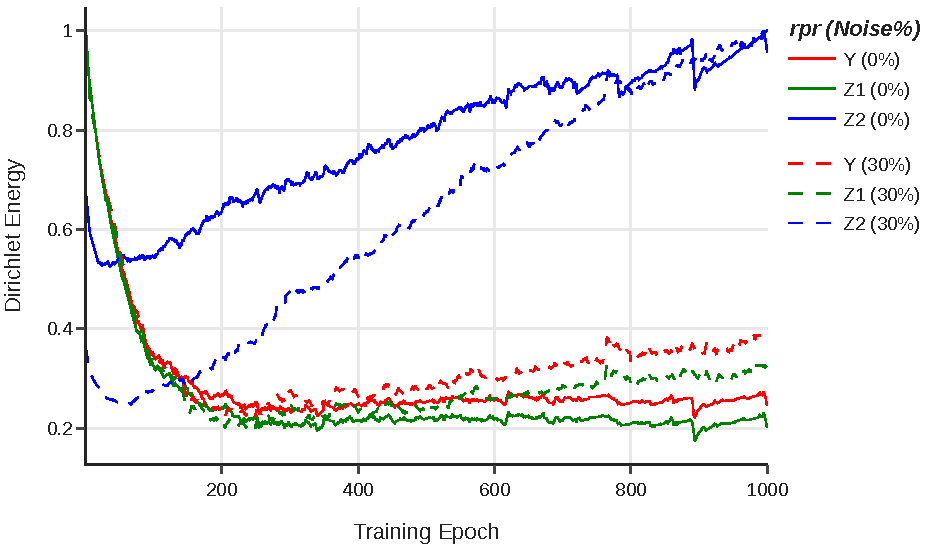
\includegraphics[width=\linewidth]{AISTATS/figures/enzymez1z2y.pdf}
    \caption{Normalized Dirichlet energy (Y, Z1, Z2)}
\end{subfigure}
\hfill
\begin{subfigure}{0.45\textwidth}
    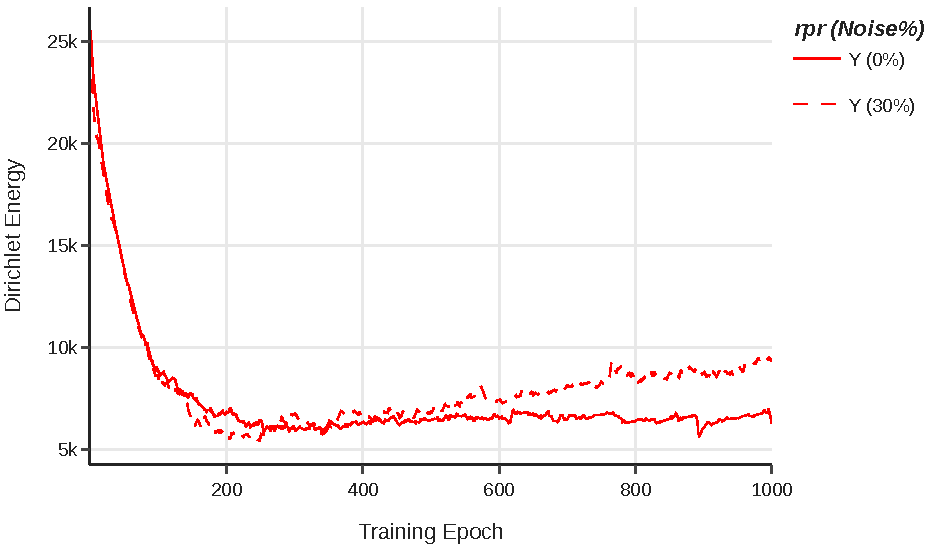
\includegraphics[width=\linewidth]{AISTATS/figures/enzymey.pdf}
    \caption{Dirichlet energy of Y}
\end{subfigure}

\vspace{1ex}

\begin{subfigure}{0.45\textwidth}
    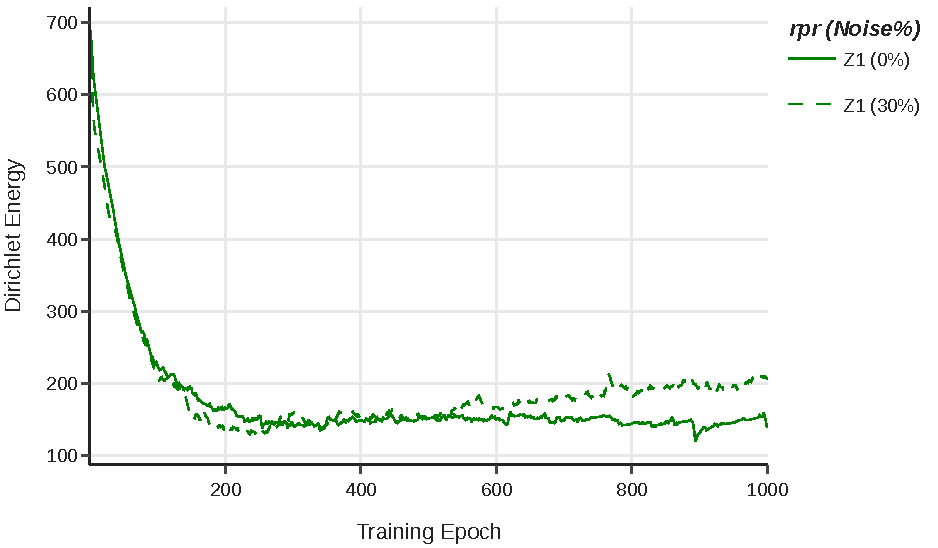
\includegraphics[width=\linewidth]{AISTATS/figures/enzymez1.pdf}
    \caption{Dirichlet energy of Z1}
\end{subfigure}
\hfill
\begin{subfigure}{0.45\textwidth}
    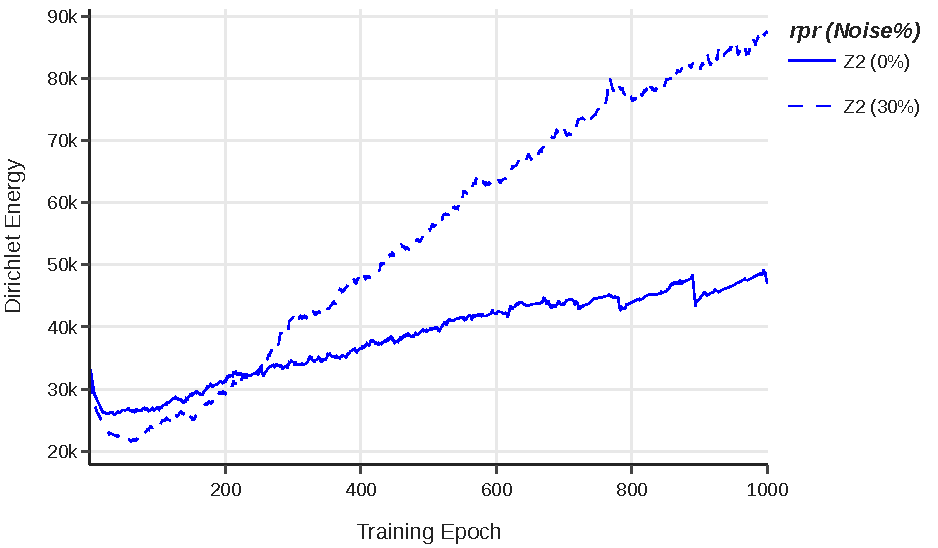
\includegraphics[width=\linewidth]{AISTATS/figures/enzymez2.pdf}
    \caption{Dirichlet energy of Z2}
\end{subfigure}

\caption{Evolution of Dirichlet energy across training epochs for the representations \( Y \), \( Z_1 \), and \( Z_2 \) learned by the FGRL model on the ENZYMES dataset. Solid lines represent training with 0\% label noise, while dashed lines correspond to 30\% symmetric label noise. The top-left plot shows the normalized energy trajectories for all three representations, with each normalized by its own maximum value to enable direct comparison. The remaining plots display the raw Dirichlet energy for each representation individually, preserving their respective scales to emphasize magnitude differences and noise sensitivity.}
\label{fig:dirichlet_energy_comparison}

\end{figure}



% \begin{figure}[htbp]
%     \centering
%     % Top-left: Normalized comparison plot
%    \begin{subfigure}[b]{0.45\textwidth}
%         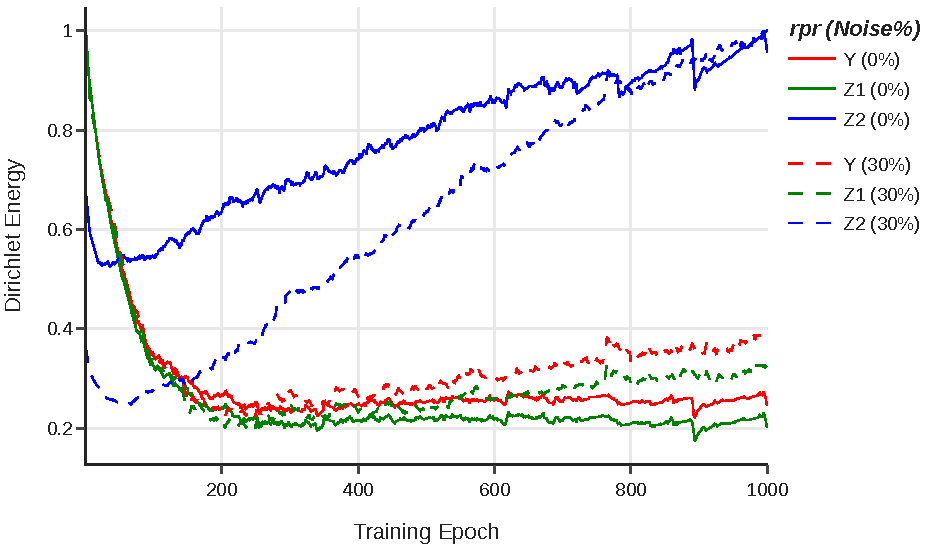
\includegraphics[width=\textwidth]{AISTATS/figures/enzymez1z2y.pdf}
%         \caption{Normalized Dirichlet energy (Y, Z1, Z2)}
%     \end{subfigure}
%     \hfill
%     \begin{subfigure}[b]{0.45\textwidth}
%         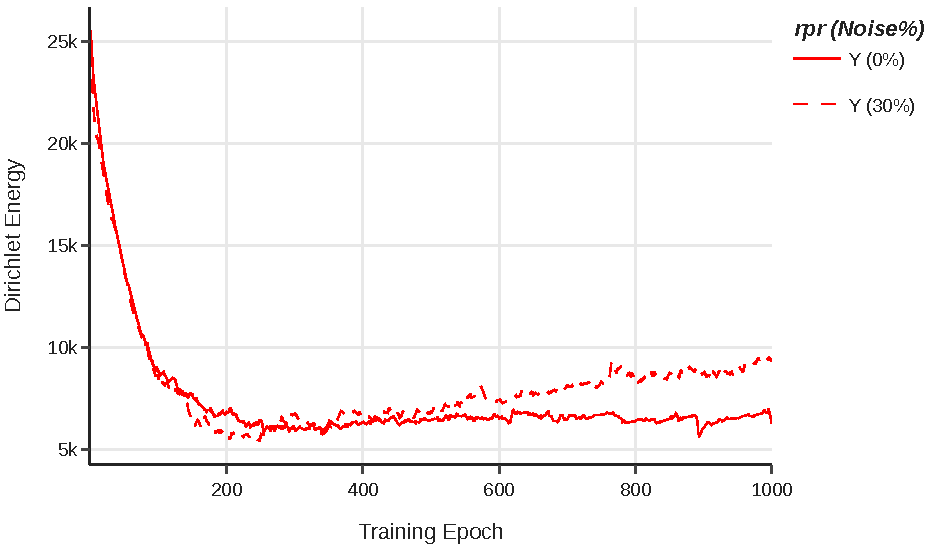
\includegraphics[width=\textwidth]{AISTATS/figures/enzymey.pdf}
%         \caption{Dirichlet energy of Y}
%     \end{subfigure}
    
%     \vskip\baselineskip
    
%     \begin{subfigure}[b]{0.45\textwidth}
%         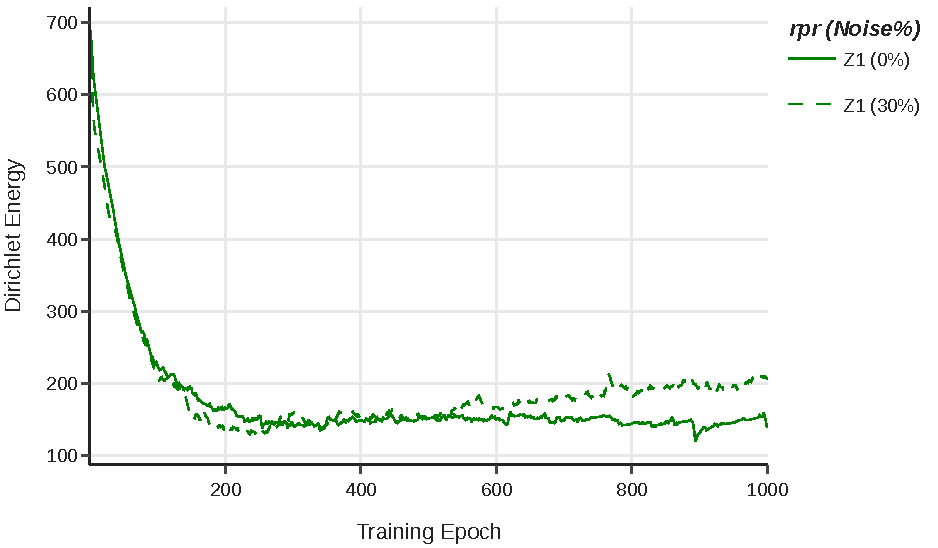
\includegraphics[width=\textwidth]{AISTATS/figures/enzymez1.pdf}
%         \caption{Dirichlet energy of Z1}
%     \end{subfigure}
%     \hfill
%     \begin{subfigure}[b]{0.45\textwidth}
%         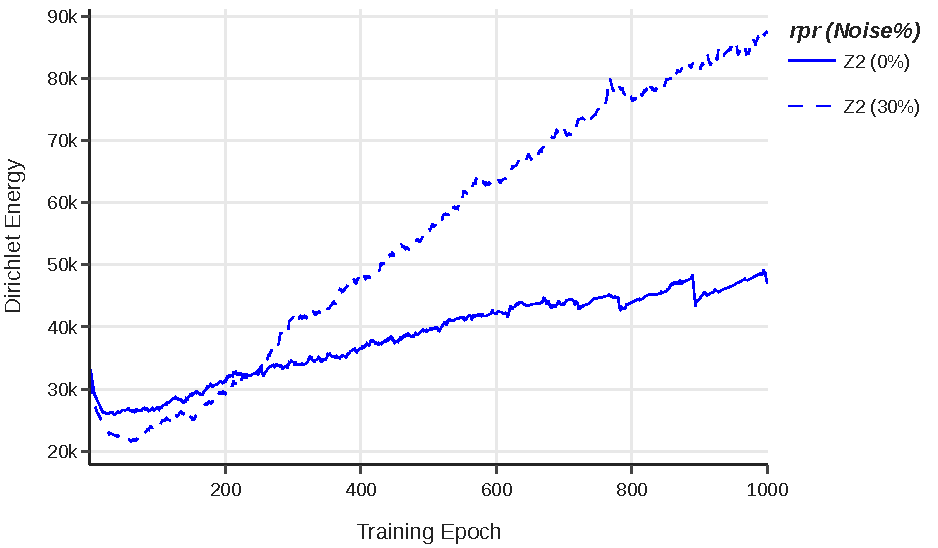
\includegraphics[width=\textwidth]{AISTATS/figures/enzymez2.pdf}
%         \caption{Dirichlet energy of Z2}
%     \end{subfigure}
    
%     \caption{%
%         Evolution of Dirichlet energy across training epochs for the representations \( Y \), \( Z_1 \), and \( Z_2 \) learned by the FGRL model on the ENZYMES dataset. Solid lines represent training with 0\% label noise, while dashed lines correspond to 30\% symmetric label noise. The top-left plot shows the normalized energy trajectories for all three representations, with each normalized by its own maximum value to enable direct comparison. The remaining plots display the raw Dirichlet energy for each representation individually, preserving their respective scales to emphasize magnitude differences and noise sensitivity.
%     }
%     \label{fig:dirichlet_energy_comparison}
% \end{figure}



Furthermore, statistical descriptors such as slope and standard deviation of \( E_{\text{dir}}(Z_2) \) were found to be strong early indicators of label noise. Under clean conditions, these metrics remained stable, but they deviated significantly under noisy labels, especially for mislabeled graphs.

These insights lead to actionable strategies for robust training:

\begin{itemize}
    \item High-frequency components (\( Z_2 \)) are principal amplifiers of label inconsistencies.
    \item Monitoring \( E^{\text{dir}}(Z_2) \) dynamics allows early identification of noise driven instability.
    \item Losses can be adaptively modulated to suppress noisy gradient propagation through \( Z_2 \).
\end{itemize}

By grounding robustness in frequency sensitive learning signals, we offer a principled mechanism that can be used to detect and curb overfitting. This analysis extends and reinforces the findings of Section~\ref{sec:Dirichlet_meet_GC}, charting a refined path forward in noise resilient GNN design.
